%%%%%%%%%%%%%%%%%%%%%%%%%%%%%%%%%%%%%%%%%%%%%%%%%%%%%%%%%%%%%%%%%%%%%%
% writeLaTeX Example: A quick guide to LaTeX
%
% Source: Dave Richeson (divisbyzero.com), Dickinson College
% 
% A one-size-fits-all LaTeX cheat sheet. Kept to two pages, so it 
% can be printed (double-sided) on one piece of paper
% 
% Feel free to distribute this example, but please keep the referral
% to divisbyzero.com
% 
%%%%%%%%%%%%%%%%%%%%%%%%%%%%%%%%%%%%%%%%%%%%%%%%%%%%%%%%%%%%%%%%%%%%%%
% How to use writeLaTeX: 
%
% You edit the source code here on the left, and the preview on the
% right shows you the result within a few seconds.
%
% Bookmark this page and share the URL with your co-authors. They can
% edit at the same time!
%
% You can upload figures, bibliographies, custom classes and
% styles using the files menu.
%
% If you're new to LaTeX, the wikibook is a great place to start:
% http://en.wikibooks.org/wiki/LaTeX
%
%%%%%%%%%%%%%%%%%%%%%%%%%%%%%%%%%%%%%%%%%%%%%%%%%%%%%%%%%%%%%%%%%%%%%%

\documentclass[10pt,landscape]{article}
\usepackage{amssymb,amsmath,amsthm,amsfonts}
\usepackage{multicol,multirow}
\usepackage{calc}
\usepackage{ifthen}
\usepackage{xcolor}
\usepackage{cancel}
\usepackage{tikz}
\usepackage{pgfplots}
\pgfplotsset{compat=1.18}
\usepackage[landscape]{geometry}
\usepackage[colorlinks=true,citecolor=blue,linkcolor=blue]{hyperref}


\ifthenelse{\lengthtest { \paperwidth = 11in}}
    { \geometry{top=.5in,left=.5in,right=.5in,bottom=.5in} }
	{\ifthenelse{ \lengthtest{ \paperwidth = 297mm}}
		{\geometry{top=1cm,left=1cm,right=1cm,bottom=1cm} }
		{\geometry{top=1cm,left=1cm,right=1cm,bottom=1cm} }
	}
\pagestyle{empty}
\makeatletter
\renewcommand{\section}{\@startsection{section}{1}{0mm}%
                                {-1ex plus -.5ex minus -.2ex}%
                                {0.5ex plus .2ex}%x
                                {\normalfont\large\bfseries}}
\renewcommand{\subsection}{\@startsection{subsection}{2}{0mm}%
                                {-1explus -.5ex minus -.2ex}%
                                {0.5ex plus .2ex}%
                                {\normalfont\normalsize\bfseries}}
\renewcommand{\subsubsection}{\@startsection{subsubsection}{3}{0mm}%
                                {-1ex plus -.5ex minus -.2ex}%
                                {1ex plus .2ex}%
                                {\normalfont\small\bfseries}}
\makeatother
\setcounter{secnumdepth}{0}
\setlength{\parindent}{0pt}
\setlength{\parskip}{0pt plus 0.5ex}
% -----------------------------------------------------------------------

\title{Algebra HSLU Kevin Häusler}

\begin{document}

\raggedright
\footnotesize

\begin{center}
    \Large{\textbf{Algebra HSLU Kevin Häusler}} \\
\end{center}
\begin{multicols}{3}
    \setlength{\premulticols}{1pt}
    \setlength{\postmulticols}{1pt}
    \setlength{\multicolsep}{1pt}
    \setlength{\columnsep}{2pt}
    \section{Zahlen und Logik}
    \subsection{Zahlen}
    \begin{tabular}{l|l|l}
        \textbf{*}         & \textbf{Bedeutung}                           & \textbf{Beispiel}                            \\ \hline
        $\mathbb{N}$       & \verb!Natürliche Zahlen = ganze Positive!    & \verb!{1;2;3;}!                              \\ \hline
        ${\mathbb{N}}_{0}$ & \verb!Natürliche Zahlen mit 0!               & \verb!{0;1;2;}!                              \\ \hline
        $\mathbb{Z}$       & \verb!Ganze Zahlen = N + ganze Negative!     & \verb!{-1;0;1;}!                             \\ \hline
        $\mathbb{Q}$       & \verb!Rationale Zahlen = Bruchzahlen!        & $\frac{3}{7} $ $\frac{5}{9} $ $\frac{2}{3} $ \\ \hline
        \verb!!            & \verb!Irrationale Zahlen = Nachkommastellen! & \verb!0.3281!                                \\ \hline
        $\mathbb{R}$       & \verb!Reele Zahlen = Q + Irrationale Zahlen! & \verb!Alle!                                  \\
    \end{tabular}

    \subsection{Mengen Operationen}
    \begin{tabular}{l|l}
        \textbf{*}                   & \textbf{Bedeutung}                               \\ \hline
        $\varnothing$ oder \verb!{}! & \verb!Leere Menge, enthält keine Elemente!       \\ \hline
        $x\in A$                     & \verb!Beschreibt Element x ist in Menge A!       \\ \hline
        $x\notin A$                  & \verb!Beschreibt Element x ist nicht in Menge A! \\ \hline
        $A\subset B$                 & \verb!A ist eine Teilmenge von B!                \\ \hline
        $A\cap B$                    & \verb!Schnittmenge von A und B!                  \\ \hline
        $A\cup B$                    & \verb!Vereinigunsgsmenge von A und B!            \\ \hline
        $A\backslash B$              & \verb!Differenzbildung, Menge von A ohne B!      \\
    \end{tabular}
    \def\firstcircle{(0,0) circle (1cm)}
    \def\secondcircle{(0:1.2cm) circle (1cm)}

    \colorlet{circle edge}{blue!50}
    \colorlet{circle area}{blue!20}

    \tikzset{filled/.style={fill=circle area, draw=circle edge, thick},
        outline/.style={draw=circle edge, thick}}

    \setlength{\parskip}{5mm}
    % Set A and B
    \begin{tikzpicture}
        \begin{scope}
            \clip \firstcircle;
            \fill[filled] \secondcircle;
        \end{scope}
        \draw[outline] \firstcircle node {$A$};
        \draw[outline] \secondcircle node {$B$};
        \node[anchor=south] at (current bounding box.north) {$A \cap B$};
    \end{tikzpicture}
    \begin{tikzpicture}
        \draw[filled] \firstcircle node {$A$}
        \secondcircle node {$B$};
        \node[anchor=south] at (current bounding box.north) {$A \cup B$};
    \end{tikzpicture}

    % Set A but not B
    \begin{tikzpicture}
        \begin{scope}
            \clip \firstcircle;
            \draw[filled, even odd rule] \firstcircle node {$A$}
            \secondcircle;
        \end{scope}
        \draw[outline] \firstcircle
        \secondcircle node {$B$};
        \node[anchor=south] at (current bounding box.north) {$A\backslash  B$};
    \end{tikzpicture}
    \begin{tikzpicture}
        \draw[filled, even odd rule] \firstcircle node {$A$}
        \secondcircle node{$B$};
        \node[anchor=south] at (current bounding box.north) {$\overline{A \cap B}$};
    \end{tikzpicture}

    \subsection{Aussagenlogik}
    \textbf{Term:}  Ein Term ist eine sinnvolle Zusammensetzung von Zahlen,
    Variablen, Operationszeichen und Klammern.
    Ein Term hat keinen Wahrheitsgehalt, ist also weder wahr noch falsch. \\[2mm]
    \textbf{Aussage:}
    Eine Aussage beschreibt durch Worte oder Zeichen einen Sachverhalt.
    Eine Aussage ist entweder wahr oder falsch. \\[2mm]
    \textbf{Aussageform:}
    Jeder sprachliche oder zeichensymbolische Ausdruck mit wenigstens einer Variablen
    wenn er durch jede sinnvolle Belegung der Variablen jeweils eine Aussage wird.
    \begin{tabular}{l|l|l}
        \textbf{*}            & \textbf{Bedeutung}                                & \textbf{Beispiel}             \\ \hline
        \verb!|A| !           & \verb!Kardinalität/Mächtigkeit beschreibt!        & \verb!A = {1;2}!              \\
                              & \verb!Anzahl Elemente einer Menge!                & \verb!|A| = 2!                \\ \hline
        $\land$               & \verb!Konkuktion/UND! A $\land$ B = Wahr wenn     & A $\land$ B                   \\
                              & A und B beide Wahr sind                           & A, B = W                      \\ \hline
        $\lor$                & \verb!Disjunktion/ODER!  A $\lor$ B  = Wahr wenn  & \verb!{-1;0;1;}!              \\
                              & A oder B  jeweils Wahr ist                        &                               \\ \hline
        $\neg$                & \verb!Negation A = Wahr! $\neg$A = Falsch         & $\neg $A                      \\\hline
        $\implies$            & Implikation: Daraus folgt                         &                               \\ \hline
        $\Longleftrightarrow$ & \verb!Äquivalenz A!  $\Longleftrightarrow$ B wenn &                               \\
                              & beide wahr oder falsch sind                       &                               \\ \hline
        $\forall$             & \verb!Für Alle!                                   & $\forall$ $x \in \mathbb{N}$  \\ \hline
        $\exists$             & \verb!Es Existiert!                               & $\exists $ $x \in \mathbb{N}$ \\ \hline
    \end{tabular}

    \begin{tabular}{@{ }c@{ }@{ }c | c@{ }@{ }c@{ }@{ }c@{ }@{ }c@{ }@{ }c | c@{ }@{ }c@{ }@{ }c@{ }@{ }c@{ }@{ }c | c@{ }@{ }c | c@{ }@{ }c@{ }@{ }c@{ }@{ }c@{ }@{ }c@{ }@{ }c}
        A & B &  & A & $\land$            & B &  &  & A & $\lor$             & B &  & $\lnot$            & B &  & A & $\lor$             & $\lnot$ & B & \\
        \hline
        T & T &  & T & \textcolor{red}{T} & T &  &  & T & \textcolor{red}{T} & T &  & \textcolor{red}{F} & T &  & T & \textcolor{red}{T} & F       & T & \\
        T & F &  & T & \textcolor{red}{F} & F &  &  & T & \textcolor{red}{T} & F &  & \textcolor{red}{T} & F &  & T & \textcolor{red}{T} & T       & F & \\
        F & T &  & F & \textcolor{red}{F} & T &  &  & F & \textcolor{red}{T} & T &  & \textcolor{red}{F} & T &  & F & \textcolor{red}{F} & F       & T & \\
        F & F &  & F & \textcolor{red}{F} & F &  &  & F & \textcolor{red}{F} & F &  & \textcolor{red}{T} & F &  & F & \textcolor{red}{T} & T       & F & \\
    \end{tabular}

    \subsection{Summe und Produkte}
    \textbf{Summezeichen:} \\
    Es sei:  n, k $\in$ Z und n $\geq$ k
    \[ \sum_{k=1}^{n} a_k = a_1 + a_2 + a_3 + \ldots + a_n \]
    k heisst Laufvariable, Laufindex oder Summationsvariable \\
    1 heisst Startwert oder untere Grenze \\
    n heisst Endwert oder obere Grenze \\
    $a_{k}$ ist die Funktion bezüglich der Laufvariable \\~\\
    \textbf{Beispiel:}
    $\sum_{k=1}^{5} k^2$

    \begin{align*} \sum_{k={\color{blue}1}}^{{\color{red}5}} k^2 &= {\color{blue}1}^2 + {\color{green}2}^2 + {\color{green}3}^2 + {\color{green}4}^2 + {\color{red}5}^2 \\ &= 1 + 4 + 9 + 16 + 25 \\[5px] &= 55 \end{align*}
    \textbf{Produktzeichen:}
    \[ \prod_{k=1}^{n} a_k = a_1 \cdot a_2 \cdot a_3 \cdot \ldots \cdot a_n\]
    k heisst Laufvariable oder Laufindex \\
    1 heisst Startwert oder untere Grenze \\
    n heisst Endwert oder obere Grenze \\
    $a_{k}$ ist die Funktion bezüglich der Laufvariable \\~\\
    \textbf{Beispiel:}
    $\prod_{k=1}^{5} k^2$ \\
    \begin{align*} \prod_{k={\color{blue}1}}^{{\color{red}5}} k^2 &= {\color{blue}1}^2 \cdot {\color{green}2}^2 \cdot {\color{green}3}^2 \cdot {\color{green}4}^2 \cdot {\color{red}5}^2 \\ &= 1 \cdot 4 \cdot 9 \cdot 16 \cdot 25 \\[5px] &= 14400 \end{align*}

    \section{Gleichungen}
    \textbf{Gleichungen Lösen} \\
    Jede Zahl aus der Definitionsmenge, die beim Einsetzen für x zu einer wahren Aussage führt, heisst Lösung der Gleichung. \\
    \textbf{Grundmenge, Definitionsbereich} $\mathbb{D}$ \\
    Die Menge aus der die Lösungen stammen dürfen. \\
    \textbf{Lösungsvariable} \\
    Variable nach der aufgelöst wird. \\
    \textbf{Formvariablen, Parameter} \\
    Alle anderen Variablen. \\
    \textbf{Lösungsmenge} \\
    Menge aller Elemente aus der Definitionsmenge, die zu einer wahren Aussage führen. \\
    \textbf{Äquivalenz} \\
    Zwei Gleichungen sind äquivalent, wenn beim Ersetzen der Variablen durch die gleichen Elemente der "gemeinsamen" Definitonsmenge entweder beide in eine wahre oder falsche Aussage übergehen. \\~\\
    \textbf{Beispiel:}
    \begin{align*} 4(x+1{,}5) &= 9x - 6 - 7x &&{\color{gray}| \text{ Terme vereinfachen}} \\[5px] 4x + 6 &= 2x - 6 &&{\color{gray}|\, -2x} \\[5px] 4x {\color{gray}\,-\,2x} + 6 &= 2x {\color{gray}\,-\,2x} - 6 \\[5px] 2x + 6 &= -6 &&{\color{gray}|\, -6} \\[5px] 2x {\color{gray}\,-\,6} &= -6 {\color{gray}\,-\,6} \\[5px] 2x &= -12 &&{\color{gray}|\, :2} \\[5px] \frac{2x}{\color{gray}2} &= \frac{-12}{\color{gray}2} \\[5px] x &= -6 &&{\color{gray}| \text{ Lösungsmenge ablesen}} \end{align*}
    \subsection{Äquivalenz­umformungen}
    Umformungen einer Gleichung, bei denen die Lösungsmenge gleich bleibt, heißen Äquivalenzumformungen. \newpage
    Folgende Äquivalenzumformungen sind möglich: \\~\\
    \textbf{1. Termunformungen}\\
    $2x+5-3=0$ $\Longleftrightarrow$
    $2x +2 = 0$ \\
    \textbf{2. Add./Sub.. mit der gleichen Zahl auf beiden Seiten} \\
    \textbf{3. Mult./Div. mit der gleichen Zahl auf beiden Seiten} \\
    Achtung: Ausser mit 0 \\
    \textbf{4. Beidseitige Add./Sub. mit dem gleichen Term} \\
    \textbf{5. Beidseitige Mult./Div. mit dem gleichen Term} \\
    \subsection{Lineare Gleichungen}
    Eine Gleichung, die sich durch Äquivalenzumformungen in die Form $ax + b = 0$
    bringen lässt, heisst lineare Gleichung. Wir können lineare Gleichungen daran erkennen, dass die Variable nur in der 1. Potenz auftritt – also kein $x^2$,$x^3$ , … enthalten. \\~\\
    \textbf{Beispiel Lösung einer linearen Gleichung}

    \begin{align*} 2 (2x - 1) &= 3 (x + 1) &&| \text{ Ausmultiplizieren} \\[5px] 4x - 2 &= 3x + 3 &&|\, -3x \\[5px] x - 2 &= 3 &&|\, +2 \\[5px] x &= 5 \end{align*}
    Lösungsmenge angeben:  $\mathbb{L} = \{5\}$ \\
    \subsection{Quadratische Gleichungen}
    Gleichungen, die sich durch Äquivalenzumformungen auf die Form $ax^2 + bx + c = 0 \quad (a, b, c \in \mathbb{R}; a \neq 0)$
    bringen lassen, heißen quadratische Gleichungen. Wir können quadratische Gleichungen daran erkennen, dass die Variable $x$ in der 2. Potenz $x^2$, aber in keiner höheren Potenz vorkommt. Es gibt 4 Arten/Formen von Quadratischen Gleichungen.\\~\\
    \textbf{Beispiel Lösung einer Reinquadratische Gleichung} \\~\\
    $ax^2 = 0$: Reinquadratische Gleichungen ohne Absolutglied besitzen als einzige Lösung die Null.
    \begin{align*} x^2 &= 0 &&{\color{gray}|\, \sqrt{\phantom{0}}} \\[5px] \sqrt{x^2} &= \pm\sqrt{0} \\[5px] x &= \pm 0 \\[5px] x &= 0 \end{align*}
    Lösungsmenge angeben:  $\mathbb{L} =  0$ \\~\\
    \textbf{Beispiel Lösung einer Reinquadratische Gleichung mit Absolutglied} \\~\\
    $x^2 - 9 = 0$ Gleichung nach $x^2$ auflösen: \\
    \begin{align*} x^2 - 9 &= 0 &&{\color{gray}|\, +9} \\[5px] x^2 - 9 {\color{gray}\;+\;9} &= 0 {\color{gray}\;+\;9} \\[5px] x^2 &= 9 \end{align*}
    Wurzel ziehen:
    \begin{align*} x^2 &= 9 &&{\color{gray}|\, \sqrt{\phantom{9}}} \\[5px] \sqrt{x^2} &= \pm\sqrt{9} \\[5px] x &= \pm 3 \end{align*}
    Fall Unterscheidung: \\
    $x_2 = 3$ , $x_2 = -3$ \\
    Lösungsmenge angeben:  $    \mathbb{L} = \{-3; 3\}$ \\~\\
    \textbf{Beispiel Lösung einer Gemischtquadratische Gleichungen ohne Absolutglied} \\~\\
    Gemischtquadratische Gleichungen ohne Absolutglied lösen wir folgendermaßen: \\
    $-2x^2 + 4x = 0$ Quadratische Gleichung in Normalform bringen: \\
    \begin{align*} -2x^2 + 4x &= 0 &&{\color{gray}|\, :(-2)} \\[5px] \frac{-2x^2 + 4x}{\color{gray}-2} &= \frac{0}{\color{gray}-2} \\[5px] \frac{-2x^2}{\color{gray}-2} + \frac{4x}{\color{gray}-2} &= \frac{0}{\color{gray}-2} \\[5px] x^2 - 2x &= 0 \end{align*}
    x ausklammern: \\
    \[x \cdot (x - 2) = 0\]
    Faktoren gleich Null setzen:\\
    \[\underbrace{x\vphantom{()}}_{=\,0} \cdot \underbrace{(x - 2)}_{=\,0} = 0\]
    Gleichungen nach x auflösen: \\
    1. Faktor: x = 0 \\
    2. Faktor:
    \begin{align*} x - 2 &= 0 &&{\color{gray}|\, +2} \\[5px] x - 2 {\color{gray}\;+\;2} &= 0 {\color{gray}\;+\;2} \\[5px] x &= 2 \end{align*}
    Lösungsmenge angeben:  $    \mathbb{L} = \{0; 2\}$ \\
    \textbf{Mitternachtsformel}\\~\\
    Gemischtquadratische Gleichungen $ax^2 + bx + c = 0$ mit Absolutglied lösen wir mit der Mitternachtsformel:\\~\\
    \[x_{1/2} = \frac{-b \pm \sqrt{b^2 - 4ac}}{2a}\]\\~\\
    Fallunterscheidung:
    \[x_{1} = \dfrac{-b - \sqrt{b^2 - 4ac}}{2a}\]
    \[x_{2} = \dfrac{-b + \sqrt{b^2 - 4ac}}{2a}\]\\~\\
    \textbf{Regeln}\\~\\
    Wenn das lineare Glied fehlt, gilt b = 0. \\
    Wenn das absolute Glied fehlt, gilt c = 0. \\
    Wenn das $x^2$ allein steht, gilt a = 0 (wegen $1 \cdot x^2 = x^2$).
    Wenn das x allein steht, gilt (wegen $1 \cdot x = x$).\\~\\
    \textbf{Lösen einer Quadratischen Gleichung mit Mitternachtsformel}\\~\\

    $2x^2 - 8x + 8 = 0$ a, b und c aus der allgemeinen Form herauslesen: \\~\\
    a = 2, b = -8 und c = 8\\~\\
    a, b und c in die Mitternachtsformel einsetzen:\\~\\
    \begin{align*} x_{1, 2} &= \frac{-b \pm \sqrt{b^2 - 4ac}}{2a} \\[5px] &= \frac{-(-8) \pm \sqrt{(-8)^2 - 4 \cdot 2 \cdot 8}}{2 \cdot 2} \end{align*}
    Lösungen berechnen: \\
    \begin{align*} \phantom{x_{1, 2}} &= \frac{8 \pm \sqrt{64 - 64}}{4} \\[5px] &= \frac{8 \pm \sqrt{{\fcolorbox{yellow}{yellow}{$0$}}}}{4} \qquad {\colorbox{yellow}{Wenn $b^2 - 4ac = 0$...}} \\[5px] &= \frac{8 \pm 0}{4} \\[5px] &= \frac{8}{4} \\[5px] &= 2 \end{align*}
    Lösungsmenge angeben:
    \[\mathbb{L} = \{2\} \quad \quad {\colorbox{yellow}{...dann gibt es eine Lösung!}}\] \newpage
    \subsection{Bruchgleichung}
    Eine Bruchgleichung ist eine Gleichung mit mindestens einem Bruchterm, in dem die Variable x im Nenner vorkommt.


    \textbf{Lösen einer Bruchgleichung}\\~\\
    \[\frac{1}{x} = \frac{2}{x+1}\]
    Definitionsmenge bestimmen: \\
    Wann wird der Nenner des Bruchs gleich Null?
    \[2x = 0 \quad \Rightarrow \quad x = 0\]
    Für wird der Nenner gleich Null. Daraus folgt: \\~\\
    1. Nenner x = 0, 2. Nenner $x + 1 = 0 \quad \Rightarrow \quad x = -1$ \\
    Defintionsmenge: $\mathbb{D} = \mathbb{R} \setminus \{-1; 0\}$ \\~\\
    Gleichung nach x auflösen. Brüche auf eine Seite bringen:
    \[\frac{1}{{\colorbox{yellow}{$x$}}} - \frac{2}{{\colorbox{orange}{$x+1$}}} = 0\]
    Brüche auf einen gemeinsamen Nenner bringen:
    \[\frac{1}{{\colorbox{yellow}{$x$}}} \cdot \frac{{\colorbox{orange}{$x+1$}}}{{\colorbox{orange}{$x+1$}}} - \frac{2}{{\colorbox{orange}{$x+1$}}} \cdot \frac{{\colorbox{yellow}{$x$}}}{{\colorbox{yellow}{$x$}}} = 0\]
    \[\frac{x+1}{x(x+1)} - \frac{2x}{x(x+1)}= 0\]
    \[\frac{(x+1) - 2x}{x(x+1)} = 0\]
    \[\frac{-x + 1}{x(x+1)} = 0\]
    Mit dem Hauptnenner multiplizieren, um den Bruch zu beseitigen:\\
    \[\frac{-x + 1}{x(x+1)} \cdot x(x+1) = 0 \cdot x(x+1)\]
    \[\frac{-x + 1}{\cancel{x(x+1)}} \cdot \cancel{x(x+1)} = 0\]
    \[-x + 1 = 0\]
    Nach x auflösen:
    \[-x + 1 = 0 \qquad |+x\]
    Prüfen, ob der x-Wert in der Definitionsmenge enthalten ist:\\
    Da x = 1 in der Definitionsmenge $\mathbb{D} = \mathbb{R} \setminus \{0\}$ liegt, haben wir eine gültige Lösung berechnet. \\~\\
    \textbf{Kehrwert}\\~\\
    Den Kehrwert eines Bruchs erhält man durch Vertauschen von Zähler und Nenner.\\~\\
    \[\frac{{\colorbox{yellow}{$1$}}}{{\colorbox{orange}{$x$}}} = \frac{{\colorbox{yellow}{$2$}}}{{\colorbox{orange}{$x+1$}}}\]
    \[\frac{{\colorbox{orange}{$x$}}}{{\colorbox{yellow}{$1$}}} = \frac{{\colorbox{orange}{$x+1$}}}{{\colorbox{yellow}{$2$}}}\]
    Umschreiben zu: $x = 0{,}5x + 0{,}5$ und auflösen zu $0{,}5x = 0{,}5 \qquad |\, \cdot 2$ $\Rightarrow x = 1$ \\~\\
    \textbf{Multiplikation übers Kreuz}\\~\\
    Wenn auf beiden Seiten der Gleichung jeweils ein Bruch steht, kann eine Multiplikation über Kreuz sinnvoll sein.
    \[\frac{{\colorbox{yellow}{$1$}}}{{\colorbox{orange}{$x$}}} = \frac{{\colorbox{orange}{$2$}}}{{\colorbox{yellow}{$x+1$}}}\]
    \[{\colorbox{yellow}{$1$}} \cdot {\colorbox{yellow}{$x+1$}} = {\colorbox{orange}{$2$}} \cdot {\colorbox{orange}{$x$}}\]
    \[x+1 = 2x \qquad |\, -x\]
    \[\Rightarrow x = 1\]
    \subsection{Betragsgleichung}
    Betragsgleichungen lassen sich durch Fallunterscheidung lösen.

    \begin{equation*} |a| = \begin{cases} a &\text{für } a \geq 0 \\[5px] -a &\text{für } a < 0 \end{cases} \end{equation*}\\~\\
    Aus der Definition des Betrags ergeben sich folgende zwei Fälle: \\
    \begin{itemize}
        \item Wenn der Term im Betrag größer oder gleich Null ist ($a \geq 0$), können wir den Term einfach ohne Betragsstriche schreiben ($|a| = a$)
        \item Wenn der Term im Betrag kleiner als Null ist ($a < 0$) , müssen wir die Vorzeichen des Terms umdrehen, um die Betragsstriche weglassen zu können ($|a| = -a$).
    \end{itemize}
    Die Lösungsmengen der einzelnen Fälle geben wir als Intervalle an. \\
    Die Lösungmenge der Gleichung ist die Vereinigungsmenge der einzelnen Lösungsmengen.\\~\\
    \textbf{Beispiel} $|x + 1| = 3$\\~\\

    Aus der Definiton des Betrag ergibt sich: \\
    \begin{equation*} |x + 1| = \begin{cases} x + 1 &\text{für } {\color{green}x + 1 \geq 0} \\[5px] -(x + 1) &\text{für } {\color{red}x + 1 < 0} \end{cases} \end{equation*}\\~\\
    Fallunterscheidung Fall 1: $x + 1\geq 0$:\\~\\
    \begin{align*} x + 1 &\geq 0 &&{\color{gray}|\, -1} \\[5px] x &\geq -1 \end{align*}\\~\\
    Fallunterscheidung Fall 2: $x + 1 < 0$:\\~\\
    \begin{align*} x + 1 &< 0 &&{\color{gray}|\, -1} \\[5px] x &< -1 \end{align*}\\~\\
    Zusammenfassung:
    \begin{equation*} |x + 1| = \begin{cases} x + 1 &\text{für } {\color{green}x \geq -1} \\[5px] -(x + 1) &\text{für } {\color{red}x < -1} \end{cases} \end{equation*}\\~\\
    \textbf{Lösungsmengen der einzelnen Fälle bestimmen:} \\
    Fall 1 $x + 1\geq 0$:\\~\\
    Für $x \geq -1$ können wir Gleichung $|x + 1| = 3$ umschreiben zu $x + 1 = 3$, Jetzt müssen wir noch die Gleichung nach x auflösen:
    \[x + 1 {\color{gray}\:-\:1} = 3 {\color{gray}\:-\:1}\]
    \[x = 2\] \\
    Die Lösungsmenge $\mathbb{L}_1$ muss sowohl die Bedingung $x \geq -1$ (1. Fall) als auch $x = 2$ (Lösung 1. Fall) erfüllen:
    \[\mathbb{L}_1 = \{2\}\]
    Fall 2: $x < -1$ \\~\\
    Für  $x < -1$ können wir Gleichung umschreiben zu $|x + 1| = 3$ \\
    Jetzt müssen wir noch die Gleichung nach x auflösen:
    \[-x - 1 = 3\]
    \[-x - 1 {\color{gray}\:+\:1} = 3 {\color{gray}\:+\:1}\]
    \[-x = 4\]
    \[-x {\color{gray}\:\cdot\:(-1)} = 4 {\color{gray}\:\cdot\:(-1)}\]
    \[x = -4\] \\~\\
    Die Lösungsmenge muss sowohl die Bedingung $x < -1$ (2. Fall) als auch $x = -4$ (Lösung 2. Fall) erfüllen:
    \[\mathbb{L}_2 = \{-4\}\]\\~\\
    \textbf{Lösungsmenge der Betragsgleichung bestimmen}\\
    \[\mathbb{L} = \mathbb{L}_1 \cup \mathbb{L}_2 = \{2\} \cup \{-4\} = \{-4; 2\}\]
    \newpage
    \subsection{Potenzgleichungen}
    Eine Potenzgleichung ist eine Gleichung, die aus nur einer Potenz einer Variable und einer Konstanten besteht: $x^n = a$ \\~\\
    Die Vorgehensweise unterscheidet sich danach, wie der Exponent n aussieht:
    \begin{enumerate}
        \item Typ: $x^n = a$ mit n $\in \mathbb{N}$
        \item Typ: $x^{-n} = a$ mit n $\in \mathbb{N}$
        \item Typ: $x^{\frac{m}{n}} = a$ mit n $\in \mathbb{N}$ und mit $m \in \mathbb{Z}$
    \end{enumerate}
    Grundsätzlich lösen wir Potenzgleichungen durch Wurzelziehen. Das Problem ist, dass das Wurzelziehen im Allgemeinen keine Äquivalenzumformung ist. Um zu verhindern, das Lösungen verloren gehen, muss man bei geraden Exponenten Betragsstriche setzen:
    \begin{itemize}
        \item Wenn n gerade ist, gilt: $\sqrt[n]{x^n} = |x|$.
        \item Wenn n ungerade ist, gilt: $\sqrt[n]{x^n} = x$.
    \end{itemize}
    \textbf{Typ 1:} $n \in \mathbb{N}$
    \begin{align*} x^2 &= 4 &&{\color{gray}|\, \sqrt{\phantom{x}}} \\[5px] \sqrt{x^2} &= \sqrt{4} &&{\color{gray}| \text{ Da $n$ gerade ist, gilt: } \sqrt[n]{x^n} = |x|} \\[5px] |x| &= 2 \\[5px] x &= \pm 2 \end{align*}
    Die Lösung der Potenzgleichung $x^2 = 0$ ist $\mathbb{L} = \{0\}$.
    \begin{align*} x^3 &= 8 &&{\color{gray}|\, \sqrt[3]{\phantom{x}}} \\[5px] \sqrt[3]{x^3} &= \sqrt[3]{8} &&{\color{gray}| \text{ Da $n$ ungerade ist, gilt: } \sqrt[n]{x^n} = x} \\[5px] x &= 2 \end{align*}
    Die Lösung der Potenzgleichung $x^3 = 8$ ist $\mathbb{L} = \{2\}$.\\~\\
    \textbf{Typ 2:} $x^{-n} = a$\\
    Vorgehensweise: Umformung der Gleichung zu Typ 1 (falls $a \neq 0$)\\
    Mögliche Lösungen
    \begin{itemize}
        \item : $a = 0$ Es gibt keine Lösung $\mathbb{L} = \{\}$.
        \item  $a \neq 0$ Die Gleichung $x^{-n} = a$ ist äquivalent zu $x^n = \frac{1}{a}$.
    \end{itemize}
    \begin{align*} x^{-2} &= 3 &&{\color{gray}| \text{ Potenzgesetz anwenden: } x^{-n} = \frac{1}{x^n}} \\[5px] \frac{1}{x^2} &= 3 &&{\color{gray}| \text{ Kehrwert}} \\[5px] x^2 &= \frac{1}{3} &&{\color{gray}|\, \sqrt{\phantom{x}}} \\[5px] \sqrt{x^2} &= \sqrt{\frac{1}{3}} &&{\color{gray}| \text{ Da $n$ gerade ist, gilt: } \sqrt[n]{x^n} = |x|} \\[5px] |x| &= \sqrt{\frac{1}{3}} \\[5px] x &= \pm \sqrt{\frac{1}{3}} \end{align*}
    Die Lösung der Potenzgleichung $x^{-2} = 3$ ist $\mathbb{L} = \left\{-\sqrt{\frac{1}{3}};+\sqrt{\frac{1}{3}}\right\}$.\\~\\
    \textbf{Typ 3:} $m \in \mathbb{Z}$ \\
    Vorgehensweise: Potenzieren mit n\\
    Ist der Exponent $\frac{m}{n}$ keine ganze Zahl, so sind die Gleichungen in $\mathbb{R}^{-}$ nicht definiert. In $\mathbb{R}_{0}^{+}$ sind die Gleichungen $x^{\frac{m}{n}} = a$ und $\sqrt[n]{x^m} = a$ äquivalent.\\~\\
    \begin{align*} x^{\frac{2}{3}} &= 4 &&{\color{gray}| \text{ Potenzieren mit 3}} \\[5px] (x^{\frac{2}{3}})^3 &= 4^3 \\[5px] x^2 &= 64 &&{\color{gray}|\, \sqrt{\phantom{x}}} \\[5px] \sqrt{x^2} &= \sqrt{64} &&{\color{gray}| \text{ Da $n$ gerade ist, gilt: } \sqrt[n]{x^n} = |x|} \\[5px] |x| &= 8 \\[5px] x &= \pm 8 \end{align*}
    $x_1 = -8$ gehört nicht zur Definitionsmenge $\mathbb{R}_{0}^{+}$.\\
    $x_2 = 8$ ist eine mögliche Lösung. Da Potenzieren i. Allg. keine Äquivalenzumformung ist, ist eine Probe unerlässlich.
    \begin{align*} x^{\frac{2}{3}} &= 4 &&{\color{gray}|\; x_2 = 8} \\[5px] {\color{red}8}^{\frac{2}{3}} &= 4 \\[5px] 4 &= 4 &&{\color{green}\phantom{|} \text{ Wahre Aussage!}} \end{align*}
    Die Lösung der Potenzgleichung $x^{\frac{2}{3}} = 4$ ist $\mathbb{L} = \{8\}$.
    \subsection{Wurzelgleichung}
    Eine Wurzelgleichung ist eine Gleichung, bei der die Variable (auch) unter einer Wurzel vorkommt. \\
    \begin{enumerate}
        \item Wurzeln beseitigen
              \begin{enumerate}
                  \item Wurzel isolieren
                  \item Potenzieren
              \end{enumerate}
        \item Algebraische Gleichung lösen
        \item Probe Machen
        \item Lösungsmenge aufschreiben
    \end{enumerate}
    \textbf{Beispiel:} $\sqrt{x + \sqrt{2x}} = 2$ \\
    Die Wurzel ist bereits isoliert, gehe direkt zu Potenzieren:
    \begin{align*} \sqrt{x + \sqrt{2x}} &= 2 &&{\color{gray}| \text{ Quadrieren}} \\[5px] \sqrt{x + \sqrt{2x}}^2 &= 2^2 \\[5px] x + \sqrt{2x} &= 4 \end{align*}
    \textbf{Wurzel isolieren:}
    \begin{align*} x + \sqrt{2x} &= 4 &&{\color{gray}|\, -x} \\[5px] \sqrt{2x} &= 4 - x \end{align*}
    \textbf{Potenzieren:}
    \begin{align*} \sqrt{2x} &= 4 - x &&{\color{gray}| \text{ Quadrieren}} \\[5px] \sqrt{2x}^2 &= (4 - x)^2 \\[5px] 2x &= 16 - 8x + x^2 \end{align*}
    \textbf{ Schritt 2: Algebraische Gleichung lösen:}\\
    Quadratische Gleichung in Normalform bringen:
    \begin{align*} 2x &= 16 - 8x + x^2 &&{\color{gray}|\, -2x} \\[5px] 0 &= 16 - 10x + x^2 &&{\color{gray}| \text{ Seiten vertauschen}} \\[5px] 16 - 10x + x^2 &= 0 &&{\color{gray}| \text{ Nach Potenzen von $x$ sortieren}} \\[5px] x^2 - 10x + 16 &= 0 \end{align*}
    Quadratische Gleichung mit der Mitternachtsformel lösen:
    \[x_{1;2}=\frac{-b\pm\sqrt{b^2-4ac}}{2a}=\qquad\color{gray}{\text{[Formel hinschreiben]}}\]
    \[=\frac{-(-10)\pm\sqrt{(-10)^2-4\cdot 1\cdot 16}}{2\cdot 1}=\qquad\color{gray}{\text{[Zahlen für a, b und c einsetzen]}}\]
    \[=\frac{10\pm\sqrt{36}}{2}\qquad\color{gray}{\text{[Nenner sowie Term innerhalb der Wurzel ausrechnen]}}\]
    \[=\frac{10\pm 6}{2}\qquad\color{gray}{\text{[Wurzel berechnen]}}\]
    Daraus folgt: \\
    $x_1=\frac{10+6}{2}=8$ und $x_2=\frac{10-6}{2}=2$\\~\\
    \textbf{Schritt 3 Probe Machen}
    \begin{align*} \sqrt{x + \sqrt{2x}} &= 2 &&{\color{gray}|\, x_1 = 2} \\[5px] \sqrt{{\color{red}2} + \sqrt{2 \cdot {\color{red}2}}} &= 2 \\[5px] \sqrt{2 + \sqrt{4}} &= 2 \\[5px] \sqrt{2 + 2} &= 2 \\[5px] \sqrt{4} &= 2 \\[5px] 2 &= 2 &&{\color{green}\phantom{|} \text{ Wahre Aussage!}} \end{align*}
    $x_1 = 2$ gehört zur Lösung der Wurzelgleichung.
    \begin{align*} \sqrt{x + \sqrt{2x}} &= 2 &&{\color{gray}|\, x_2 = 8} \\[5px] \sqrt{{\color{red}8} + \sqrt{2 \cdot {\color{red}8}}} &= 2 \\[5px] \sqrt{8 + \sqrt{16}} &= 2 \\[5px] \sqrt{8 + 4} &= 2 \\[5px] \sqrt{12} &= 2 &&{\color{red}\phantom{|} \text{ Falsche Aussage!}} \end{align*}
    $x_2 = 8$ ist offensichtlich nur eine Scheinlösung. \\~\\
    \textbf{Schritt 4 Lösungsmenge aufschreiben}\\
    $\mathbb{L} = \{2\}$
    \subsection{Exponential­gleichungen}
    Eine Exponentialgleichung ist eine Gleichung, in der die Variable im Exponenten einer Potenz steht. \\~\\
    \textbf{Lösung durch Logarithmieren Beispiel 1}\\~\\
    \[a^{f(x)} = b^{g(x)} \quad \Rightarrow \quad f(x) \cdot \log a = g(x) \cdot \log b\]\\~\\
    Löse $2^x = 9$.\\
    \begin{align*} 2^x &= 9 &&{\color{orange}| \text{ Logarithmieren}} \\[5px] \log 2^x &= \log 9 &&{\color{gray}| \text{ Exponent vorziehen}} \\[5px] x \cdot \log 2 &= \log 9 &&{\color{gray}|\, :\log 2} \\[5px] x &= \frac{\log 9}{\log 2} &&{\color{gray}| \text{ Taschenrechner!}} \\[5px] x &\approx 3{,}1699 && \Rightarrow \mathbb{L} = \{3{,}1699\} \end{align*}
    \textbf{Lösung durch Logarithmieren Beispiel 2}\\~\\
    \[a^{f(x)} = b^{g(x)} \quad \Rightarrow \quad f(x) \cdot \log a = g(x) \cdot \log b\]\\~\\
    Löse $2^{x+3} = 3^x$. \\
    \begin{align*} 2^{x+3} &= 3^x &&{\color{orange}| \text{ Logarithmieren}} \\[5px] \log 2^{x+3} &= \log 3^x &&{\color{gray}| \text{ Exponent vorziehen}} \\[5px] (x+3) \cdot \log 2 &= x \cdot \log 3 &&{\color{gray}| \text{ Klammer ausmulti}} \\[5px] x \cdot \log 2 + 3 \cdot \log 2 &= x \cdot \log 3 &&{\color{gray}|\, -(x \cdot \log 2)} \\[5px] 3 \cdot \log 2 &= x \cdot \log 3 - x \cdot \log 2 &&{\color{gray}|\, x \text{ ausklammern}} \\[5px] 3 \cdot \log 2 &= x \cdot (\log 3 - \log 2) &&{\color{gray}|\, : (\log 3 - \log 2)} \\[5px] x &= \frac{3 \cdot \log 2}{\log 3 - \log 2} &&{\color{gray}| \text{ Taschenrechner!}} \\[5px] x &\approx 5{,}1285 && \Rightarrow \mathbb{L} = \{5{,}1285\} \end{align*}
    \subsection{Logarithmus­gleichungen}
    Eine Logarithmusgleichung ist eine Gleichung, in der die Variable im Numerus des Logarithmus steht. \\~\\
    \textbf{Lösung mithilfe der Definition des Logarithmus}\\~\\
    Eine Lösung mithilfe der Definition des Logarithmus ist nur dann möglich, wenn es gelingt, die Terme auf beiden Seiten der Gleichung so umzuformen, dass sich auf der einen Seite ein Logarithmus und auf der anderen Seite eine Konstante ergeben.
    \begin{align*} \log_{2}x &= 3 &&{\color{orange}| \text{ Anwendung der Definition des Logarithmus}} \\[5px] x &= 2^3 &&{\color{gray}| \text{ Potenz ausrechnen}} \\[5px] x &= 8 && \Rightarrow \mathbb{L} = \{8\} \end{align*}
    \begin{align*} 2 \cdot \log_{4}x &= 2 &&{\color{gray}|\, :2} \\[5px] \log_{4}x &= 1 &&{\color{orange}| \text{ Anwendung der Definition des Logarithmus}} \\[5px] x &= 4^1 &&{\color{gray}| \text{ Potenz ausrechnen}} \\[5px] x &= 4 && \Rightarrow \mathbb{L} = \{4\} \end{align*}
    \begin{align*} \log_{3}9 + \log_{3}x &= 4 &&{\color{gray}| \text{ Logarithmen zusammenfassen}} \\[5px] \log_{3}9x &= 4 &&{\color{orange}| \text{ Anwendung der Definition des Logarithmus}} \\[5px] 9x &= 3^4 &&{\color{gray}| \text{ Potenz ausrechnen}} \\[5px] 9x &= 81 &&{\color{gray}|\, :9} \\[5px] x &= 9 && \Rightarrow \mathbb{L} = \{9\} \end{align*}\\~\\
    \textbf{Definitionsmenge einer Logarithmusgleichung }\\~\\
    Da $\log_{b}x = a$  nur für $x > 0$ definiert ist, kann die Definitionsmenge eingeschränkt sein.

    In der Praxis bedeutet das, dass wir stets die Probe machen sollten, d.h. überprüfen, ob die berechneten Lösungen eingesetzt in die gegebene Gleichung zu einer wahren Aussage führen.\\~\\
    \begin{align*} 2 \cdot \log_{7}x &= \log_{7}16 &&{\color{gray}|\text{ Faktor beseitigen}} \\[5px] \log_{7}x^2 &= \log_{7}16 &&{\color{orange}|\text{ Numerivergleich}} \\[5px] x^2 &= 16 &&{\color{gray}|\text{ Wurzel ziehen}} \\[5px] x &= \pm \sqrt{16} &&{\color{gray}|\text{ Wurzel berechnen}} \\[5px] x &= \pm 4 \\[5px] \end{align*}
    Als Lösungen erhalten wir $x_1 = -4$ und $x_2 = +4$.\\~\\

    Da $\log_{b}x = a$ nur für $x > 0$ definiert ist, ist $x_1 = -4$ nur eine \textbf{Scheinlösung.}\\~\\

    Die einzige Lösung der Logarithmusgleichung ist $x_2 = 4$:\\
    \[\Rightarrow \mathbb{L} = \{4\}\]
    \section{Lineare Gleichungs­systeme}
    Mehrere lineare Gleichungen, die alle zusammen gelten sollen, bilden ein lineares Gleichungssystem.\\
    \subsection{Gleichsetzungsverfahren}
    \begin{enumerate}
        \item Gleichungen nach der gleichen Variable auflösen
        \item Gleichungen gleichsetzen
        \item Gleichung nach der enthaltenen Variable auflösen
        \item Berechneten Wert in eine der umgeformten Gleichungen aus Schritt 1 einsetzen und zweiten Wert berechnen
        \item Lösungsmenge aufschreiben
    \end{enumerate}
    \textbf{Beispiel LGS mit Gleichsetzungsverfahren}\\~\\
    \begin{align*} 2x + 3y &= 14 \\ x + 2y &= 8 \end{align*}
    \textbf{Schritt 1 Gleichungen nach der gleichen Variable auflösen}\\~\\
    Wir entscheiden uns dafür, die Gleichungen nach x aufzulösen. \\
    1. Gleichung:
    \[2x + 3y = 14 \qquad |\, {\color{red}-3y}\]
    \[2x + 3y {\color{red}\: - \: 3y} = 14 {\color{red}\: - \: 3y}\]
    \[2x = 14 - 3y \qquad |\, :{\color{orange}2}\]
    \[\frac{2x}{{\color{orange}2}} = \frac{14 - 3y}{{\color{orange}2}}\]
    \[{\colorbox{yellow}{$x = 7 - 1{,}5y$}}\]
    2. Gleichung:
    \[x + 2y = 8 \qquad |\, {\color{red}-2y}\]
    \[x + 2y {\color{red}\: - \: 2y} = 8 {\color{red}\: - \: 2y}\]
    \[{\colorbox{orange}{$x = 8 - 2y$}}\]
    \textbf{Schritt 2 Gleichungen gleichsetzen}\\~\\
    Es gilt ${\colorbox{yellow}{$x$}} = {\colorbox{orange}{$x$}}$ bzw. ${\colorbox{yellow}{$7 - 1{,}5y$}} = {\colorbox{orange}{$8 - 2y$}}$\\~\\
    \textbf{Schritt 3 Gleichung nach der enthaltenen Variable auflösen}\\~\\
    Wir lösen die Gleichung nach y auf
    \[7 - 1{,}5y = 8 - 2y \qquad |\, {\color{red}+2y}\]
    \[7 - 1{,}5y {\color{red} \: + \: 2y} = 8 - 2y {\color{red}\: + \: 2y}\]
    \[7 + 0{,}5y = 8 \qquad |\, {\color{orange}-7}\]
    \[7 {\color{orange} \: - \: 7} + 0{,}5y = 8 {\color{orange}\: - \: 7}\]
    \[0{,}5y = 1 \qquad |\, :{\color{red}0{,}5}\]
    \[\frac{0{,}5y}{{\color{red}0{,}5}} = \frac{1}{{\color{red}0{,}5}}\]
    \[y = 2\]
    \textbf{Schritt 4 Berechneten Wert in eine der umgeformten Gleichungen aus Schritt 1 einsetzen und zweiten Wert berechnen}\\~\\
    Wenn $y = 2$ wir entweder in die Gleichung ${\colorbox{yellow}{$x = 7 - 1{,}5y$}}$ oder in die Gleichung ${\colorbox{orange}{$x = 8 - 2y$}}$  einsetzen, so erhalten wir den zweiten Wert $x = 4$ \\~\\
    \textbf{Schritt 5 Lösungsmenge aufschreiben}
    \[\mathbb{L} = \{(4|2)\}\]
    \subsection{Einsetzungsverfahren}
    \begin{enumerate}
        \item     Eine Gleichung nach einer Variable auflösen
        \item     Berechneten Term für diese Variable in die andere Gleichung einsetzen
        \item     Gleichung nach der enthaltenen Variable auflösen
        \item     Berechneten Wert in die umgeformte Gleichung aus Schritt 1 einsetzen und zweiten Wert berechnen
        \item     Lösungsmenge aufschreiben
    \end{enumerate}
    \textbf{Beispiel LGS mit Einsetzugnsverfahren}\\~\\
    \begin{align*} 2x + 3y &= 14 \\ x + 2y &= 8 \end{align*}
    \textbf{Schritt 1 Eine Gleichung nach einer Variable auflösen}\\~\\
    Wir entscheiden uns dafür, die 2. Gleichung nach x aufzulösen, da wir dafür nur 2y subtrahieren müssen.
    \[x + 2y = 8 \qquad |\, {\color{red}-2y}\]
    \[x + 2y {\color{red}\: - \: 2y} = 8 {\color{red}\: - \: 2y}\]
    \[x = {\colorbox{yellow}{$8 - 2y$}}\]
    \textbf{Schritt 2 Berechneten Term für diese Variable in die andere Gleichung einsetzen}\\~\\
    Wir setzen $x = {\colorbox{yellow}{$8 - 2y$}}$ in die 1. Gleichung
    \[2x + 3y = 14\]
    ein und erhalten
    \[2 \cdot ({\colorbox{yellow}{$8 - 2y$}}) + 3y = 14\]
    \textbf{Schritt 3 Gleichung nach der enthaltenen Variable auflösen}\\~\\
    Wir lösen die Gleichung nach y auf
    \[2 \cdot (8 - 2y) + 3y = 14\]
    \[16 - 4y + 3y = 14\]
    \[16 - y = 14 \qquad |\, {\color{red}-16}\]
    \[16 {\color{red}\: - \: 16} - y = 14 {\color{red}\: - \: 16}\]
    \[-y = -2 \qquad |\, {\color{orange}\cdot (-1)}\]
    \[-y {\color{orange}\: \cdot \: (-1)} = -2 {\color{orange} \: \cdot \: (-1)}\]
    \[y = 2\]
    \textbf{Schritt 4 Berechneten Wert in die umgeformte Gleichung aus Schritt 1 einsetzen und zweiten Wert berechnen}\\~\\
    Die umgeformte Gleichung aus Schritt 1 ist
    \[{\colorbox{yellow}{$x = 8 - 2y$}}\]
    In diese Gleichung setzen wir $y = 2$ ein
    \[x = 8 - 2 \cdot 2\]
    \[x = 4\]
    \textbf{Schritt 5 Lösungsmenge aufschreiben}\\~\\
    \[\mathbb{L} = \{(4|2)\}\]
    \subsection{Additions­verfahren}
    \begin{enumerate}
        \item     Gleichungen so umformen, dass die Koeffizienten einer Variablen Gegenzahlen werden
        \item     Gleichungen addieren
        \item     Gleichung nach der enthaltenen Variable auflösen
        \item     Berechneten Wert in eine der ursprünglichen Gleichungen einsetzen und zweiten Wert berechnen
        \item     Lösungsmenge aufschreiben
    \end{enumerate}
    Damit die Koeffizienten der Variablen Gegenzahlen werden, bilden wir das kleinste gemeinsame Vielfache (kgV) der Koeffizienten und formen die Gleichungen anschließend entsprechend um.
    \textbf{Beispiel LGS mit Additionsverfahren}\\~\\
    \begin{align*} 2x + 3y &= 14 \\ x + 2y &= 8 \end{align*}
    \textbf{Schritt 1 Gleichungen so umformen, dass die Koeffizienten einer Variablen Gegenzahlen werden}\\~\\
    Wir entscheiden uns dafür, die Koeffizienten der Variable x zu Gegenzahlen zu machen. Dazu bilden wir das kleinste gemeinsame Vielfache (kgV) der Koeffizienten von x:
    \[\text{kgV}(1;2) = 2\]
    Damit in einer Gleichung eine 2 und in der anderen Gleichung eine -2 vor dem x steht, müssen wir lediglich die 2. Gleichung mit -2 multiplizieren:
    \begin{align*} 2x + 3y &= 14 \\ x + 2y &= 8 \qquad |\, \cdot (-2) \end{align*}
    \begin{align*} 2x + 3y &= 14 \\ -2x - 4y &= -16 \end{align*}
    \newpage
    \textbf{Schritt 2 Gleichungen addieren}\\~\\
    Jetzt addieren wir die beiden Gleichungen, wodurch die Variable x eliminiert wird. Übrig bleibt:
    \[-y = -2\]
    \textbf{Schritt 3 Gleichung nach der enthaltenen Variable auflösen}\\~\\
    Wir lösen die eben berechnete Gleichung nach auf, indem wir mit -1 multiplizieren:
    \[-y = -2 \qquad |\, {\color{orange}\cdot (-1)}\]
    \[-y {\color{orange} \: \cdot \: (-1)} = -2 {\color{orange} \: \cdot \: (-1)}\]
    \[y = 2\]
    \textbf{Schritt 4 Berechneten Wert in eine der ursprünglichen Gleichungen einsetzen und zweiten Wert berechnen}\\~\\
    Wir setzen y=2 in eine der beiden ursprünglichen Gleichungen ein, um x zu berechnen:
    \begin{align*} 2x + 3 \cdot 2 &= 14 \\ x + 2 \cdot 2 &= 8 \end{align*}
    Unabhängig davon, welche der beiden Gleichungen wir nach x auflösen, das Ergebnis ist dasselbe:
    \[x = 4\]
    \textbf{Schritt 5 Lösungsmenge aufschreiben}\\~\\
    \[\mathbb{L} = \{(4|2)\}\]
    \section{Ungleichungen}
    Eine Ungleichung ist ein mathematischer Ausdruck, der aus zwei Termen besteht, die durch eines der Vergleichszeichen < (Kleinerzeichen), $\leq$ (Kleinergleichzeichen),
    > (Größerzeichen) oder $\geq$ (Größergleichzeichen) verbunden sind.
    \subsection{Lineare Ungleichungen}
    \begin{enumerate}
        \item Ungleichung nach x auflösen
        \item Lösungsmenge aufschreiben
    \end{enumerate}
    \begin{itemize}
        \item Terme auf beiden Seiten der Ungleichung zusammenfassen
        \item Denselben Term auf beiden Seiten der Ungleichung addieren/subtrahieren
        \item Beide Seiten der Ungleichung mit derselben positiven* Zahl multiplizieren
        \item Beide Seiten der Ungleichung durch dieselbe positive* Zahl dividieren
    \end{itemize}
    * Bei der Multiplikation bzw. Division mit einer negativen Zahl müssen wir das Ungleichungszeichen umdrehen.\\~\\
    \textbf{Beispiel:}\\~\\
    \[x - 3 \leq 3 (x-1) + 5\]
    \textbf{Schritt 1 Ungleichung nach x auflösen}\\
    \[x - 3 \leq {\color{red}3} (x-1) + 5\]
    \[x - 3 \leq {\color{red}3} \cdot x + {\color{red}3} \cdot (-1) + 5\]
    \[x - 3 \leq 3x - 3 + 5\]
    zusammenfassen
    \[x - 3 \leq 3x + 2\]
    Ungleichung nach x auflösen
    \[x {\color{red}\:-\:3x} - 3 \leq 3x {\color{red}\:-\:3x} + 2\]
    \[-2x - 3 \leq 2\]
    \[-2x - 3 {\color{red}\:+\:3} \leq 2 {\color{red}\:+\:3}\]
    \[-2x \leq 5\]
    Um die Lösung zu erhalten, müssen wir durch -2 dividieren.
    Zur Erinnerung: Bei der Division durch eine negative Zahl dreht sich das Ungleichheitszeichen um!
    \[\frac{-2x}{{\color{red}-2}} \geq \frac{5}{{\color{red}-2}}\]
    \[x \geq \frac{5}{-2}\]
    oder in Dezimalschreibweise
    \[x \geq -2{,}5\]
    \textbf{Schritt 2 Lösungsmenge aufschreiben}\\
    \[\mathbb{L} = \left[-2{,}5;\infty\right[\]
    \section{Funktionen}
    Eine Funktion $f$ ist eine Zuordnung, bei der jedem Element x der Definitionsmenge D genau ein Element y der Wertemenge W zugeordnet ist.
    \begin{tabular}{l|l}
        \textbf{Symbol}     & \textbf{Bedeutung}                         \\ \hline
        $f$                 & Name der Funktion                          \\ \hline
        $x$                 & Argument, x-Wert, unabhängige Variable     \\  \hline
        $y$                 & Funktionswert, y-Wert, abhängige Variable  \\  \hline
        $y = f(x)$          & Funktionsgleichung, Zuordnungsvorschrift*! \\ \hline
        D oder $\mathbb{D}$ & Definitionsmenge, Definitionsbereich       \\  \hline
        W oder$\mathbb{W}$  & Wertemenge, Wertebereich                   \\  \hline
    \end{tabular}
    \subsection{Lineare Funktionen}
    Eine Funktion $f$ mit der Funktionsgleichung $f(x) = mx + n$ heisst lineare Funktion. \\
    Wegen $y = f(x)$ können wir statt $f(x) = mx + n$ auch $y = mx + n$ schreiben:
    \begin{itemize}
        \item $y$: Abhängige Variable, y-Wert, Funktionswert
        \item $m$: Steigung
        \item  $x$: Unabhängige Variable, x-Wert, (Funktions-)Argument
        \item $n$ : y-Achsenabschnitt
    \end{itemize}
    Wenn wir den y-Achsenabschnitt n in $f(x) = mx + n$ verändern, passiert Folgendes:
    \begin{itemize}
        \item Gilt $n > 0$, ist die Gerade nach oben verschoben.
        \item Gilt $n < 0$ , ist die Gerade nach unten verschoben.
    \end{itemize}

    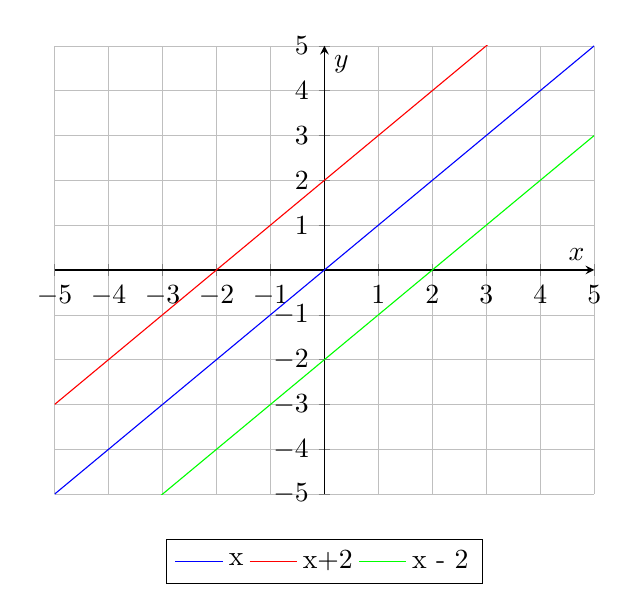
\begin{tikzpicture}%[scale=1.0]
        \begin{axis}[
                xlabel=$x$,
                ylabel=$y$,
                xmax=5,
                xmin=-5,
                ymax=5,
                ymin=-5,
                axis x line=middle,
                axis y line=middle,
                legend style={at={(0.5,-0.1)},
                        anchor=north,legend columns=-1},
                grid=major,
                grid style={line width=.1pt, draw=gray!10},
                major grid style={line width=.2pt,draw=gray!50},
                xtick={-5,-4,-3,-2,-1,0,1,2,3,4,5},
                ytick={-5,-4,-3,-2,-1,0,1,2,3,4,5}
            ]
            \addplot [blue] {x};
            \addlegendentry {x};
            \addplot [red] {x+2};
            \addlegendentry {x+2};
            \addplot [green] {x-2};
            \addlegendentry {x - 2};
        \end{axis}
    \end{tikzpicture}\\~\\
    Wenn wir die Steigungt m in $f(x) = mx + n$ verändern, passiert Folgendes:
    \begin{itemize}
        \item Gilt $m > 0$, steigt die Gerade.
        \item Gilt $m < 0$ , fällt die Gerade.
    \end{itemize}

    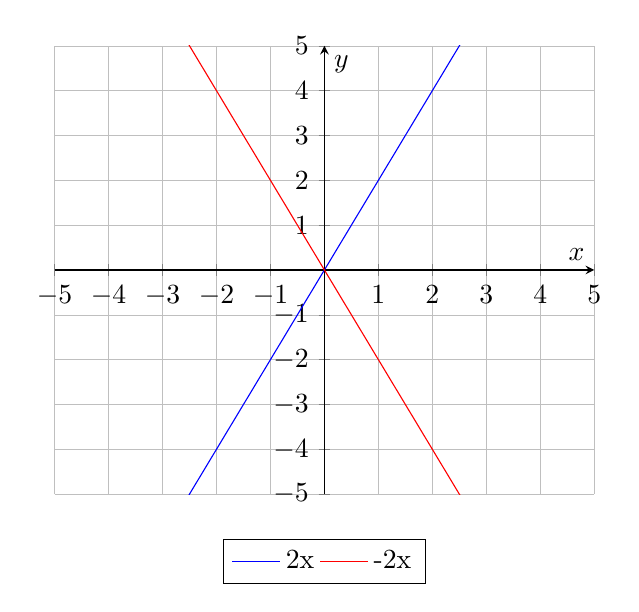
\begin{tikzpicture}%[scale=1.0]
        \begin{axis}[
                xlabel=$x$,
                ylabel=$y$,
                xmax=5,
                xmin=-5,
                ymax=5,
                ymin=-5,
                axis x line=middle,
                axis y line=middle,
                legend style={at={(0.5,-0.1)},
                        anchor=north,legend columns=-1},
                grid=major,
                grid style={line width=.1pt, draw=gray!10},
                major grid style={line width=.2pt,draw=gray!50},
                xtick={-5,-4,-3,-2,-1,0,1,2,3,4,5},
                ytick={-5,-4,-3,-2,-1,0,1,2,3,4,5}
            ]
            \addplot [blue] {x*2};
            \addlegendentry {2x};
            \addplot [red] {x*-2};
            \addlegendentry {-2x};
        \end{axis}
    \end{tikzpicture}
    \subsubsection{Nulltstelle berechnen}
    Berechne die Nullstelle der linearen Funktion  $y = 3x + 3$. \\~\\
    Wir setzen die Funktion gleich Null, d.h. wir setzen für den y Wert 0 ein: ${\color{red}{0}} = 3x + 3$ \\~\\

    Jetzt müssen wir die Gleichung nach x auflösen, um die gesuchte Nullstelle zu finden:
    \begin{align*} &3x + 3 = 0 &&|\, {\color{red}{\: - \: 3}} \\[5px] &3x + 3 {\color{red}{\: - \: 3}} = {\color{red}{\: - \: 3}} \\[5px] &3x = -3 &&|\, :{\color{red}{3}} \\[5px] &\frac{3x}{{\color{red}{3}}} = \frac{-3}{{\color{red}{3}}} \\[5px] &{\fcolorbox{red}{red}{$x = -1$}} \end{align*}
    \subsubsection{Steigung berechnen}
    Wir lesen zwei beliebige Punkte ab:
    \[P_0({\color{blue}0}|{\color{red}1}) \text{ und } P_1({\color{blue}4}|{\color{red}3})\]
    und setzen sie in die Steigungsformel ein:
    \begin{align*} m &= \frac{y_1 - y_0}{x_1 - x_0} \\[5px] &= \frac{{\color{red}3} - ({\color{red}1})}{{\color{blue}4} - {\color{blue}0}}\\[5px] &= \frac{2}{4} \\[5px] &= \frac{1}{2} \end{align*}
    \subsubsection{Schnittpunkt berechnen}
    Ein Schnittpunkt existiert nur, wenn die beiden gegebenen Geraden eine unterschiedliche Steigung besitzen.
    \[g\colon~y = {\color{red}2}x + 1\]
    \[h\colon~y = {\color{red}2}x + 3\]
    Die Geraden besitzen dieselbe Steigung. \textbf{Es existiert kein Schnittpunkt}.
    \begin{enumerate}
        \item Funktionsgleichungen gleichsetzen
        \item Gleichung nach x auflösen
        \item x in eine der beiden Funktionsgleichungen einsetzen, um y zu berechnen
        \item Ergebnis aufschreiben
    \end{enumerate}
    Berechne den Schnittpunkt der beiden Geraden $y = \frac{1}{2}x - 1$ und $y = -2x - 6$.\\~\\
    \textbf{Schritt 1 Funktionsgleichungen gleichsetzen:}\\~\\
    \[\frac{1}{2}x - 1 = -2x - 6\]
    \textbf{Schritt 2 Gleichung nach x auflösen:}\\~\\
    \begin{align*} \frac{1}{2}x - 1 &= -2x - 6 &&|\, {\color{red}+2x} \\[5px] \frac{1}{2}x {\color{red}\: + \: 2x} - 1 &= -2x {\color{red}\: + \: 2x} - 6 \\[5px] 2{,}5x - 1 &= - 6 &&|\, {\color{orange}+1} \\[5px] 2{,}5x - 1 {\color{orange}\: + \: 1} &= - 6 {\color{orange}\: + \: 1} \\[5px] 2{,}5x &= -5 &&|\, {\color{red}:2{,}5} \\[5px] \frac{2{,}5x}{{\color{red}2{,}5}} &= \frac{-5}{{\color{red}2{,}5}} \\[5px] x &= {\colorbox{yellow}{$-2$}} \end{align*}
    \textbf{Schritt 3 x in eine der beiden Funktionsgleichungen einsetzen, um y zu berechnen:}\\~\\
    Wir setzen x = -2 in die erste Gleichung ein:
    \begin{align*} y &= \frac{1}{2}x - 1 \\[5px] &= \frac{1}{2} \cdot (-2) - 1 \\[5px] &= {\colorbox{orange}{$-2$}} \end{align*}
    \textbf{Schritt 4 Ergebnis aufschreiben:}\\~\\
    Die beiden Geraden schneiden sich im Punkt $S({\colorbox{yellow}{$-2$}}|{\colorbox{orange}{$-2$}})$
    \subsubsection{Umkehrfunktion bilden}
    \begin{enumerate}
        \item Funktionsgleichung nach x auflösen
        \item x und y vertauschen
    \end{enumerate}
    Bilde die Umkehrfunktion von $f\colon\; y = 2x + 1$.\\~\\
    \textbf{Schritt 1 Funktionsgleichung nach x auflösen:}
    \begin{align*} y &= 2x + 1 &&{\color{gray}|\, -1} \\[5px] y - 1 &= 2x &&{\color{gray}|\, :2} \\[5px] \frac{1}{2}y - \frac{1}{2} &= x &&{\color{gray}| \text{ Seiten vertauschen}} \\[5px] x &= \frac{1}{2}y - \frac{1}{2} \end{align*}
    \textbf{Schritt 2 x und y vertauschen:}\\~\\
    \[ y = \frac{1}{2}x - \frac{1}{2}\]
    Die Umkehrfunktion der Funktion $f\colon\; y = 2x + 1$ ist $f^{-1}\colon\; y = 0{,}5x - 0{,}5$.\\~\\
    Um die Graphen von $f$ und $f^{-1}$ ordentlich zu zeichnen, fertigen wir zwei Wertetabellen an.
    \[\phantom{^{-1}}f\colon\; \begin{array}{r|c|c|c|c|c} x & -2 & -1 & 0 & 1 & 2 \\ \hline y & -3 & -1 & 1 & 3 & 5 \end{array}\]
    Die Wertetabelle von $f^{-1}$ erhält man durch Vertauschen der Zeilen der Wertetabelle von  $f$.
    \[f^{-1}\colon\; \begin{array}{r|c|c|c|c|c} x & -3 & -1 & 1 & 3 & 5 \\ \hline y & -2 & -1 & 0 & 1 & 2 \end{array}\]



    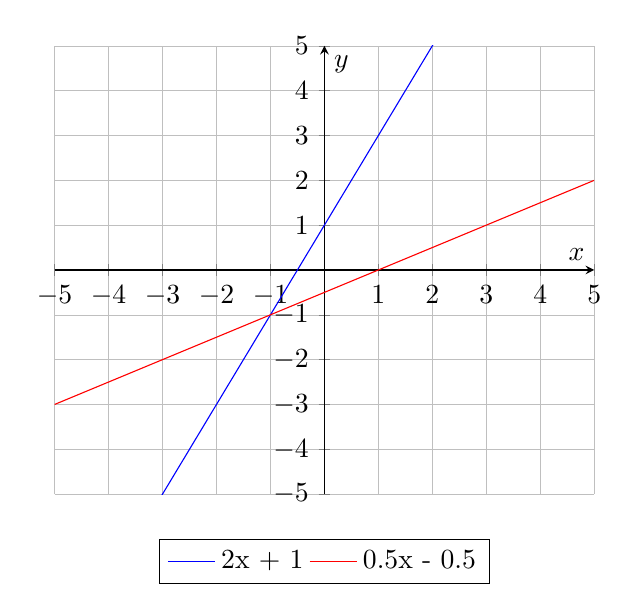
\begin{tikzpicture}%[scale=1.0]
        \begin{axis}[
                xlabel=$x$,
                ylabel=$y$,
                xmax=5,
                xmin=-5,
                ymax=5,
                ymin=-5,
                axis x line=middle,
                axis y line=middle,
                legend style={at={(0.5,-0.1)},
                        anchor=north,legend columns=-1},
                grid=major,
                grid style={line width=.1pt, draw=gray!10},
                major grid style={line width=.2pt,draw=gray!50},
                xtick={-5,-4,-3,-2,-1,0,1,2,3,4,5},
                ytick={-5,-4,-3,-2,-1,0,1,2,3,4,5}
            ]
            \addplot [blue] {x*2+1};
            \addlegendentry {2x + 1};
            \addplot [red] {x*0.5-0.5};
            \addlegendentry {0.5x - 0.5};
        \end{axis}
    \end{tikzpicture}
    \LaTeX (usually pronounced ``LAY teck,'' sometimes ``LAH teck,'' and never ``LAY tex'') is a mathematics typesetting program that is the standard for most professional mathematics writing. It is based on the typesetting program \TeX\ created by Donald Knuth of Stanford University (his first version appeared in 1978). Leslie Lamport was responsible for creating \LaTeX\, a more user friendly version of \TeX. A team of \LaTeX\ programmers created the current version,  \LaTeX\ 2$\varepsilon$.

    \section{Math vs. text vs. functions}
    In properly typeset mathematics  variables appear in italics (e.g., $f(x)=x^{2}+2x-3$). The exception to this rule is predefined functions (e.g., $\sin (x)$). Thus it is important to \textbf{always} treat text, variables, and functions correctly. See the difference between $x$ and x, -1 and $-1$, and $sin(x)$ and $\sin(x)$.
    \[ \alpha Z \frac{1}{2}\]
    There are two ways to present a mathematical expression--- \emph{inline} or as an \emph{equation}.

    \subsection{Inline mathematical expressions}
    Inline expressions occur in the middle of a sentence.  To produce an inline expression, place the math expression between dollar signs (\verb!$!).  For example, typing \verb!$90^{\circ}$ is the same as $\frac{\pi}{2}$ radians!  yields $90^{\circ}$ is the same as $\frac{\pi}{2}$ radians.

    \subsection{Equations}
    Equations are mathematical expressions that are given their own line and are centered on the page.  These are usually used for important equations that deserve to be showcased on their own line or for large equations that cannot fit inline. To produce an inline expression, place the mathematical expression  between the symbols  \verb!\[! and \verb!\]!. Typing \verb!\[x=\frac{-b\pm\sqrt{b^2-4ac}}{2a}\]! yields \[x=\frac{-b\pm\sqrt{b^2-4ac}}{2a}.\]

    \subsection{Displaystyle}
    To get full-sized inline mathematical expressions  use  \verb!\displaystyle!. Use this sparingly. Typing \verb!I want this $\displaystyle \sum_{n=1}^{\infty}! \verb!\frac{1}{n}$, not this $\sum_{n=1}^{\infty}! \verb!\frac{1}{n}$.! yields\\ I want  this $\displaystyle \sum_{n=1}^{\infty}\frac{1}{n}$, not this $\sum_{n=1}^{\infty}\frac{1}{n}.$


    \section{Images}

    You can put images (pdf, png, jpg, or gif) in your document. They need to be in the same location as your .tex file when you compile the document. Omit   \verb![width=.5in]! if you want the image to be full-sized.

    \verb!\begin{figure}[ht]!\\
    \verb!\includegraphics[width=.5in]{imagename.jpg}!\\
    \verb!\caption{The (optional) caption goes here.}!\\
    \verb!\end{figure}!


    \subsection{Text decorations}

    Your text can be \textit{italics} (\verb!\textit{italics}!), \textbf{boldface} (\verb!\textbf{boldface}!), or \underline{underlined} (\verb!\underline{underlined}!).

    Your math can contain boldface, $\mathbf{R}$ (\verb!\mathbf{R}!), or blackboard bold, $\mathbb{R}$ (\verb!\mathbb{R}!). You may want to used these to express the sets of real numbers ($\mathbb{R}$ or $\mathbf{R}$), integers ($\mathbb{Z}$ or $\mathbf{Z}$), rational numbers ($\mathbb{Q}$ or $\mathbf{Q}$), and natural numbers ($\mathbb{N}$ or $\mathbf{N}$).

    To have text appear in a math expression use \verb!\text!. \verb!(0,1]=\{x\in\mathbb{R}:x>0\text{ and }x\le 1\}! yields $(0,1]=\{x\in\mathbb{R}:x>0\text{ and }x\le 1\}$. (Without the \verb!\text! command it treats ``and'' as three variables: $(0,1]=\{x\in\mathbb{R}:x>0 and x\le 1\}$.)



    \section{Spaces and new lines}

    \LaTeX\ ignores extra spaces and new lines. For example,

    \verb!This   sentence will       look!

    \verb!fine after      it is     compiled.!

    This   sentence will       look
    fine after      it is     compiled.


    Leave one full empty line between two paragraphs. Place \verb!\\! at the end of a line to create a new line (but not create a new paragraph).

    \verb!This!

    \verb!compiles!

    ~

    \verb!like\\!

    \verb!this.!

    This
    compiles

    like\\
    this.

    Use  \verb!\noindent! to prevent a paragraph from indenting.

    \section{Comments}

    Use \verb!%! to create a comment. Nothing on the line after the \verb!%! will be typeset. \verb!$f(x)=\sin(x)$ %this is the sine function! yields $f(x)=\sin(x)$%this is the sine function

    \section{Delimiters}

    \begin{tabular}{lll}
        \emph{description} & \emph{command} & \emph{output} \\
        parentheses        & \verb!(x)!     & (x)           \\
        brackets           & \verb![x]!     & [x]           \\
        curly braces       & \verb!\{x\}!   & \{x\}         \\
    \end{tabular}

    To make your delimiters large enough to fit the content, use them together with \verb!\right! and \verb!\left!. For example, \verb!\left\{\sin\left(\frac{1}{n}\right)\right\}_{n}^! \verb!{\infty}! produces\\ $\displaystyle \left\{\sin\left(\frac{1}{n}\right)\right\}_{n}^{\infty}$.

    Curly braces are non-printing characters that are used to gather text that has more than one character. Observe the differences between the four expressions \verb!x^2!, \verb!x^{2}!, \verb!x^2t!, \verb!x^{2t}! when typeset: $x^2$, $x^{2}$, $x^2t$, $x^{2t}$.


    \section{Lists}

    You can produce ordered and unordered lists.

    \begin{tabular}{lll}
        \emph{description}          & \emph{command} & \emph{output} \\
        unordered list              &
        \begin{tabular}{l}
            \verb!\begin{itemize}! \\
            \verb!  \item!         \\
            \verb!  Thing 1!       \\
            \verb!  \item!         \\
            \verb!  Thing 2!       \\
            \verb!\end{itemize}!
        \end{tabular}   &
        \begin{tabular}{l}
            $\bullet$ Thing 1 \\
            $\bullet$ Thing 2
        \end{tabular}                                            \\
        ~                                                            \\
        ordered list                &
        \begin{tabular}{l}
            \verb!\begin{enumerate}! \\
            \verb!  \item!           \\
            \verb!  Thing 1!         \\
            \verb!  \item!           \\
            \verb!  Thing 2!         \\
            \verb!\end{enumerate}!
        \end{tabular} &
        \begin{tabular}{l}
            1.~Thing 1 \\
            2.~Thing 2
        \end{tabular}
    \end{tabular}


    \section{Symbols (in \emph{math} mode)}

    \subsection{The basics}
    \begin{tabular}{lll}
        \emph{description}       & \emph{command}      & \emph{output}   \\
        addition                 & \verb!+!            & $+$             \\
        subtraction              & \verb!-!            & $-$             \\
        plus or minus            & \verb!\pm!          & $\pm$           \\
        multiplication (times)   & \verb!\times!       & $\times$        \\
        multiplication (dot)     & \verb!\cdot!        & $\cdot$         \\
        division symbol          & \verb!\div!         & $\div$          \\
        division (slash)         & \verb!/!            & $/$             \\
        circle plus              & \verb!\oplus!       & $\oplus$        \\
        circle times             & \verb!\otimes!      & $\otimes$       \\
        equal                    & \verb!=!            & $=$             \\
        not equal                & \verb!\ne!          & $\ne$           \\
        less than                & \verb!<!            & $<$             \\
        greater than             & \verb!>!            & $>$             \\
        less than or equal to    & \verb!\le!          & $\le$           \\
        greater than or equal to & \verb!\ge!          & $\ge$           \\
        approximately equal to   & \verb!\approx!      & $\approx$       \\
        infinity                 & \verb!\infty!       & $\infty$        \\
        dots                     & \verb!1,2,3,\ldots! & $1,2,3,\ldots$  \\
        dots                     & \verb!1+2+3+\cdots! & $1+2+3+\cdots$  \\
        fraction                 & \verb!\frac{a}{b}!  & $\frac{a}{b}$   \\
        square root              & \verb!\sqrt{x}!     & $\sqrt{x}$      \\
        $n$th root               & \verb!\sqrt[n]{x}!  & $\sqrt[n]{x}$   \\
        exponentiation           & \verb!a^b!          & $a^{b}$         \\
        subscript                & \verb!a_b!          & $a_{b}$         \\
        absolute value           & \verb!|x|!          & $|x|$           \\
        natural log              & \verb!\ln(x)!       & $\ln(x)$        \\
        logarithms               & \verb!\log_{a}b!    & $\log_{a}b$     \\
        exponential function     & \verb!e^x=\exp(x)!  & $e^{x}=\exp(x)$ \\
        degree                   & \verb!\deg(f)!      & $\deg(f)$       \\
    \end{tabular}
    \newpage

    \subsection{Functions}
    \begin{tabular}{lll}
        \emph{description} & \emph{command}       & \emph{output}                                                                 \\
        maps to            & \verb!\to!           & $\to$                                                                         \\
        composition        & \verb!\circ!         & $\circ$                                                                       \\
        piecewise          & \verb!|x|=!          & \multirow{5}{*}{$\displaystyle |x|=\begin{cases}x&x\ge 0\\-x&x<0\end{cases}$} \\
        function           & \verb!\begin{cases}! &                                                                               \\
                           & \verb!x & x\ge 0\\!  &                                                                               \\
                           & \verb!-x & x<0!      &                                                                               \\
                           & \verb!\end{cases}!   &
    \end{tabular}

    \subsection{Greek and Hebrew letters}
    \begin{tabular}{llll}
        \emph{command}     & \emph{output} & \emph{command}  & \emph{output} \\
        \verb!\alpha!      & $\alpha$      & \verb!\tau!     & $\tau$        \\
        \verb!\beta!       & $\beta$       & \verb!\theta!   & $\theta$      \\
        \verb!\chi!        & $\chi$        & \verb!\upsilon! & $\upsilon$    \\
        \verb!\delta!      & $\delta$      & \verb!\xi!      & $\xi$         \\
        \verb!\epsilon!    & $\epsilon$    & \verb!\zeta!    & $\zeta$       \\
        \verb!\varepsilon! & $\varepsilon$ & \verb!\Delta!   & $\Delta$      \\
        \verb!\eta!        & $\eta$        & \verb!\Gamma!   & $\Gamma$      \\
        \verb!\gamma!      & $\gamma$      & \verb!\Lambda!  & $\Lambda$     \\
        \verb!\iota!       & $\iota$       & \verb!\Omega!   & $\Omega$      \\
        \verb!\kappa!      & $\kappa$      & \verb!\Phi!     & $\Phi$        \\
        \verb!\lambda!     & $\lambda$     & \verb!\Pi!      & $\Pi$         \\
        \verb!\mu!         & $\mu$         & \verb!\Psi!     & $\Psi$        \\
        \verb!\nu!         & $\nu$         & \verb!\Sigma!   & $\Sigma$      \\
        \verb!\omega!      & $\omega$      & \verb!\Theta!   & $\Theta$      \\
        \verb!\phi!        & $\phi$        & \verb!\Upsilon! & $\Upsilon$    \\
        \verb!\varphi!     & $\varphi$     & \verb!\Xi!      & $\Xi$         \\
        \verb!\pi!         & $\pi$         & \verb!\aleph!   & $\aleph$      \\
        \verb!\psi!        & $\psi$        & \verb!\beth!    & $\beth$       \\
        \verb!\rho!        & $\rho$        & \verb!\daleth!  & $\daleth$     \\
        \verb!\sigma!      & $\sigma$      & \verb!\gimel!   & $\gimel$
    \end{tabular}


    \subsection{Set theory}
    \begin{tabular}{lll}
        \emph{description}           & \emph{command}               & \emph{output}                           \\
        set brackets                 & \verb!\{1,2,3\}!             & $\{1,2,3\}$                             \\
        element of                   & \verb!\in!                   & $\in$                                   \\
        not an element of            & \verb!\not\in!               & $\not\in$                               \\
        subset of                    & \verb!\subset!               & $\subset$                               \\
        subset of                    & \verb!\subseteq!             & $\subseteq$                             \\
        not a subset of              & \verb!\not\subset!           & $\not\subset$                           \\
        contains                     & \verb!\supset!               & $\supset$                               \\
        contains                     & \verb!\supseteq!             & $\supseteq$                             \\
        union                        & \verb!\cup!                  & $\cup$                                  \\
        intersection                 & \verb!\cap!                  & $\cap$                                  \\
        big union                    &
        \verb!\bigcup_{n=1}^{10}A_n! &
        $\displaystyle \bigcup_{n=1}^{10}A_{n}$                                                               \\
        big intersection             & \verb!\bigcap_{n=1}^{10}A_n! & $\displaystyle \bigcap_{n=1}^{10}A_{n}$ \\
        empty set                    & \verb!\emptyset!             & $\emptyset$                             \\
        power set                    & \verb!\mathcal{P}!           & $\mathcal{P}$                           \\
        minimum                      & \verb!\min!                  & $\min$                                  \\
        maximum                      & \verb!\max!                  & $\max$                                  \\
        supremum                     & \verb!\sup!                  & $\sup$                                  \\
        infimum                      & \verb!\inf!                  & $\inf$                                  \\
        limit superior               & \verb!\limsup!               & $\limsup$                               \\
        limit inferior               & \verb!\liminf!               & $\liminf$                               \\
        closure                      & \verb!\overline{A}!          & $\overline{A}$
    \end{tabular}

    \subsection{Calculus}
    \begin{tabular}{lll}
        \emph{description}                              & \emph{command}                                & \emph{output}                      \\
        derivative                                      & \verb!\frac{df}{dx}!                          & $\displaystyle \frac{df}{dx}$      \\
        derivative                                      & \verb!\f'!                                    & $f'$                               \\
        partial derivative                              &
        \begin{tabular}{l}
            \verb!\frac{\partial f}! \\ \verb!{\partial x}!
        \end{tabular} & $\displaystyle \frac{\partial f}{\partial x}$                                                                        \\
        integral                                        & \verb!\int!                                   & $\displaystyle\int$                \\
        double integral                                 & \verb!\iint!                                  & $\displaystyle\iint$               \\
        triple integral                                 & \verb!\iiint!                                 & $\displaystyle\iiint$              \\
        limits                                          & \verb!\lim_{x\to \infty}!                     & $\displaystyle \lim_{x\to \infty}$ \\
        summation                                       &
        \verb!\sum_{n=1}^{\infty}a_n!                   &
        $\displaystyle \sum_{n=1}^{\infty}a_n$                                                                                               \\
        product                                         &
        \verb!\prod_{n=1}^{\infty}a_n!                  &
        $\displaystyle \prod_{n=1}^{\infty}a_n$
    \end{tabular}




    \subsection{Logic}
    \begin{tabular}{lll}
        \emph{description}  & \emph{command}         & \emph{output}     \\
        not                 & \verb!\sim!            & $\sim$            \\
        and                 & \verb!\land!           & $\land$           \\
        or                  & \verb!\lor!            & $\lor$            \\
        if...then           & \verb!\to!             & $\to$             \\
        if and only if      & \verb!\leftrightarrow! & $\leftrightarrow$ \\
        logical equivalence & \verb!\equiv!          & $\equiv$          \\
        therefore           & \verb!\therefore!      & $\therefore$      \\
        there exists        & \verb!\exists!         & $\exists$         \\
        for all             & \verb!\forall!         & $\forall$         \\
        implies             & \verb!\Rightarrow!     & $\Rightarrow$     \\
        equivalent          & \verb!\Leftrightarrow! & $\Leftrightarrow$
    \end{tabular}

    \subsection{Linear algebra}
    \begin{tabular}{lll}
        \emph{description}           & \emph{command}              & \emph{output}                  \\
        vector                       & \verb!\vec{v}!              & $\vec{v}$                      \\
        vector                       & \verb!\mathbf{v}!           & $\mathbf{v}$                   \\
        norm                         & \verb!||\vec{v}||!          & $||\vec{v}||$                  \\
        matrix                       &
        \begin{tabular}{l}
            \verb!\left[!             \\
            \verb!\begin{array}{ccc}! \\
            \verb!1 & 2 & 3 \\!       \\
            \verb!4 & 5 & 6\\!        \\
            \verb!7 & 8 & 0!          \\
            \verb!\end{array}!        \\
            \verb!\right]!\end{tabular} &
        $\displaystyle \left[\begin{array}{ccc}1 & 2 & 3 \\4 & 5 & 6 \\7 & 8 & 0\end{array}\right]$ \\
        \\determinant&
        \begin{tabular}{l}
            \verb!\left|!             \\
            \verb!\begin{array}{ccc}! \\
            \verb!1 & 2 & 3 \\!       \\
            \verb!4 & 5 & 6 \\!       \\
            \verb!7 & 8 & 0!          \\
            \verb!\end{array}!        \\
            \verb!\right|!
        \end{tabular} &
        $\displaystyle \left|\begin{array}{ccc}1 & 2 & 3 \\4 & 5 & 6 \\7 & 8 & 0\end{array}\right|$ \\
        determinant                  & \verb!\det(A)!              & $ \det(A)$                     \\
        trace                        & \verb!\operatorname{tr}(A)! & $\operatorname{tr}(A)$         \\
        dimension                    & \verb!\dim(V)!              & $\dim(V)$                      \\
    \end{tabular}

    \subsection{Number theory}
    \begin{tabular}{lll}
        \emph{description}      & \emph{command}            & \emph{output}        \\
        divides                 & \verb!|!                  & $|$                  \\
        does not divide         & \verb!\not |!             & $\not |$             \\
        div                     & \verb!\operatorname{div}! & $\operatorname{div}$ \\
        mod                     & \verb!\mod!               & $\operatorname{mod}$ \\
        greatest common divisor & \verb!\gcd!               & $\gcd$               \\
        ceiling                 & \verb!\lceil x \rceil!    & $\lceil x\rceil$     \\
        floor                   & \verb!\lfloor x \rfloor!  & $\lfloor x \rfloor$  \\
    \end{tabular}




    \subsection{Geometry and trigonometry}
    \begin{tabular}{lll}
        \emph{description} & \emph{command}       & \emph{output}   \\
        angle              & \verb!\angle ABC!    & $\angle ABC$    \\
        degree             & \verb!90^{\circ}!    & $90^{\circ}$    \\
        triangle           & \verb!\triangle ABC! & $\triangle ABC$ \\
        segment            & \verb!\overline{AB}! & $\overline{AB}$ \\
        sine               & \verb!\sin!          & $\sin$          \\
        cosine             & \verb!\cos!          & $\cos$          \\
        tangent            & \verb!\tan!          & $\tan$          \\
        cotangent          & \verb!\cot!          & $\cot$          \\
        secant             & \verb!\sec!          & $\sec$          \\
        cosecant           & \verb!\csc!          & $\csc$          \\
        inverse sine       & \verb!\arcsin!       & $\arcsin$       \\
        inverse cosine     & \verb!\arccos!       & $\arccos$       \\
        inverse tangent    & \verb!\arctan!       & $\arctan$       \\
    \end{tabular}

    \section{Symbols (in \emph{text} mode)}

    The followign symbols do \textbf{not} have to be surrounded by dollar signs.

    \begin{tabular}{lll}
        \emph{description} & \emph{command}        & \emph{output}  \\
        dollar sign        & \verb!\$!             & \$             \\
        percent            & \verb!\%!             & \%             \\
        ampersand          & \verb!\&!             & \&             \\
        pound              & \verb!\#!             & \#             \\
        backslash          & \verb!\textbackslash! & \textbackslash \\
        left quote marks   & \verb!``!             & ``             \\
        right quote marks  & \verb!''!             & ''             \\
        single left quote  & \verb!`!              & `              \\
        single right quote & \verb!'!              & '              \\
        hyphen             & \verb!X-ray!          & X-ray          \\
        en-dash            & \verb!pp. 5--15!      & pp. 5--15      \\
        em-dash            & \verb!Yes---or no?!   & Yes---or no?
    \end{tabular}

    \section{Resources}
    Great symbol look-up site: \href{http://detexify.kirelabs.org/}{Detexify}\\
    \href{http://amath.colorado.edu/documentation/LaTeX/Symbols.pdf}{\LaTeX\ Mathematical Symbols}\\
    \href{ftp://tug.ctan.org/pub/tex-archive/info/symbols/comprehensive/symbols-letter.pdf}{The Comprehensive \LaTeX\ Symbol List}\\
    \href{http://mirrors.med.harvard.edu/ctan/info/lshort/english/lshort.pdf}{The Not So Short Introduction to \LaTeX\ 2$\varepsilon$}\\
    \href{http://www.tug.org/}{TUG: The \TeX\ Users Group}\\
    \href{http://www.ctan.org/}{CTAN: The Comprehensive \TeX\ Archive Network}\\
    ~\\
    \LaTeX\ for the Mac: \href{http://www.tug.org/mactex/}{Mac\TeX}\\
    \LaTeX\ for the PC: \href{http://www.texniccenter.org/}{{\TeX}nicCenter} and \href{http://miktex.org/}{MiK\TeX}\\
    \LaTeX\ online: \href{http://www.writelatex.com/}{WriteLaTeX}.
    \vfill
    \hrule
    ~\\
    Dave Richeson, Dickinson College, \href{http://divisbyzero.com/}{http://divisbyzero.com/}
\end{multicols}

\end{document}